\documentclass[11pt]{article}

\usepackage[T1]{fontenc}
\usepackage[margin=1in]{geometry}
\usepackage{amsmath,amssymb,mathtools,amsthm}
\usepackage{booktabs,tabularx,array}
% microtype font expansion requires a scalable T1 font; fall back if lmodern is absent.
\IfFileExists{lmodern.sty}
  {\usepackage{lmodern}\usepackage{microtype}}
  {\usepackage[expansion=false]{microtype}}
\usepackage{enumitem}
\usepackage{tikz}
\usepackage{pgfplots}
\pgfplotsset{compat=1.16}
\usepackage[hidelinks]{hyperref}

\setlength{\parindent}{0pt}
\setlength{\parskip}{0.65em}
\setlist[itemize]{leftmargin=*,itemsep=0.2em,topsep=0.3em}
\setlist[enumerate]{leftmargin=*,itemsep=0.3em,topsep=0.3em}
\renewcommand{\arraystretch}{1.18}
\setcounter{tocdepth}{1}

\newcommand{\AP}{\operatorname{AP}}
\newcommand{\CAP}{\operatorname{CAP}}
\newcommand{\Regime}{\mathcal{R}}
\newcommand{\Tpi}{\CAP_{\pi_\star}}
\newcommand{\E}{\mathbb{E}}
\newcommand{\iid}{\mathrel{\overset{\mathrm{iid}}{\sim}}}

% Full notation, used at the point of definition.
\newcommand{\RCAPfull}{\operatorname{R\text{-}CAP}^{\mathrm{sup}}_{\Regime,\pi_\star}}
\newcommand{\RCAPHatFull}{\widehat{\operatorname{R\text{-}CAP}}{}^{\,\mathrm{sup}}_{\Regime,\pi_\star}}
% Reduced notation, used in running text once the regime is fixed.
\newcommand{\RCAP}{\operatorname{R\text{-}CAP}^{\mathrm{sup}}_{\pi_\star}}
\newcommand{\RCAPHat}{\widehat{\operatorname{R\text{-}CAP}}{}^{\,\mathrm{sup}}_{\pi_\star}}
\newcommand{\RCAPHatB}{\widehat{\operatorname{R\text{-}CAP}}{}^{\,\mathrm{sup}}_{\pi_\star,B}}
\newcommand{\RCAPnull}{\operatorname{R\text{-}CAP}^{\mathrm{sup,null}}_{\pi_\star}}
\newcommand{\RCAPnullHat}{\widehat{\operatorname{R\text{-}CAP}}{}^{\,\mathrm{sup,null}}_{\pi_\star}}
\newcommand{\RCAPcal}{\operatorname{R\text{-}CAP}_{\pi_\star}}
\newcommand{\RCAPcalHat}{\widehat{\operatorname{R\text{-}CAP}}_{\pi_\star}}

\newcommand{\PRep}{P_{\mathrm{rep}}^{\Regime,\pi_\star}}
\newcommand{\PRepHat}{\widehat{P}_{\mathrm{rep}}^{\Regime,\pi_\star}}

\newtheorem{definition}{Definition}
\newtheorem{proposition}{Proposition}
\theoremstyle{remark}
\newtheorem*{remark}{Remark}

\title{Supported Predictive Performance\\
\large A Replication-Based Extension of Chance-Corrected Average Precision}
\author{Marcus A. Thomas}
\date{Methodological proposal}

\begin{document}

\maketitle

\begin{abstract}
AUROC measures ranking discrimination without describing how many selected cases are positive. Precision--recall evaluation supplies that information. Average precision gives a finite-sample summary, although its value depends on positive-class prevalence and one evaluation may provide weak support for the observed result. A declared reference prevalence $\pi_\star$ and chance correction define an average-precision scale indexed by $\pi_\star$. A declared evaluation-generating regime $\Regime$ specifies the target population, the size and class-count design of a complete repeated evaluation, contextual conditions, sampling and dependence structure, measurement process, model-development stages, and sources of variation that may recur. Let $\Theta_{\pi_\star}$ denote the chance-corrected average precision produced by one independent execution of $\Regime$ and evaluated at $\pi_\star$. Replication-adjusted chance-corrected average precision is
\[
\RCAPfull
=
\E\!\left[
\min\{\Theta_{\pi_\star,1},\Theta_{\pi_\star,2}\}
\right].
\]
The minimum is the greatest performance level that survives both results. Its expectation over the regime summarizes location and does not state a probability, and it equals expected repeated performance minus half the expected absolute disagreement between repetitions. For a fixed model evaluated on independent or held-out data, the default estimate uses a stratified $n$-out-of-$n$ bootstrap that preserves the observed positive and negative counts in every replicate. Other sampling structures implement broader declared regimes.

Analytic chance correction places population random ranking at zero, but neither of the two finite-sample distortions acting on the metric vanishes at realistic evaluation sizes: non-interpolated average precision is upward biased under random ranking, and the minimum applies a downward disagreement penalty. The two partially cancel, with a design-dependent residual that can carry either sign. The chance level is therefore measured rather than assumed, using a permutation null executed under the same declared regime. A complete report leads with the calibrated score $\RCAPcal$, the primary reportable quantity, which restores zero to chance and one to perfect separation and is comparable across designs; it is reported together with the observed effect $\Tpi(D_{\mathrm{obs}})$ and the estimated supported effect $\RCAPHat$ that define it and fix its scale. The reference prevalence specifies the population in which selected-set purity is evaluated, the regime specifies what constitutes a repeated evaluation, and the permutation null specifies where the resulting scale begins.
\end{abstract}

\begingroup
\small
\setlength{\parskip}{0pt}
\tableofcontents
\endgroup
\newpage

\section{A sequence of evaluation problems}

When a ranking model selects cases for follow-up, evaluation must describe both separation between the classes and the composition of the selected set. AUROC addresses the first question. It is the probability that a randomly selected positive case receives a higher score than a randomly selected negative case, with ties conventionally receiving half credit. When the class-conditional score distributions remain fixed, AUROC is unchanged by positive-class prevalence.

Selection decisions require another quantity. AUROC does not state what fraction of selected cases are positive. Its false-positive rate divides false positives by the total number of negative cases. In a population with many negatives, a small false-positive rate can still yield many false positives. Strong discrimination can therefore coexist with a selected set in which most cases are negative.

Precision describes the purity of the selected set:
\[
\operatorname{Precision}
=
\frac{\operatorname{TP}}{\operatorname{TP}+\operatorname{FP}}.
\]
Recall describes the fraction of positive cases selected:
\[
\operatorname{Recall}
=
\frac{\operatorname{TP}}{\operatorname{TP}+\operatorname{FN}}.
\]
A precision--recall curve traces these quantities as the score threshold is lowered. It records how many positive cases are retrieved and how many selected cases are truly positive.

Area under the precision--recall curve, or AUPRC, is a general name for a scalar summary of this curve. Average precision, or AP, is the finite-sample rule used here:
\[
\AP
=
\sum_k (r_k-r_{k-1})p_k.
\]
Each gain in recall receives the precision at the threshold that produced it. Equal scores enter together, and no interpolation is added between observed operating points. Appendix~\ref{app:prevalence} gives the complete finite-sample definition and explains how this convention differs from other AUPRC calculations.

Precision solves the selected-set-purity problem by incorporating the number of negatives that enter the selected set. This makes precision depend on positive-class prevalence. Suppose a threshold selects $80\%$ of positive cases and $5\%$ of negative cases. Write these class-conditional selection rates as
\[
r=0.8,
\qquad
f=0.05.
\]
If half of the population is positive, precision at this threshold is
\[
\frac{0.5(0.8)}{0.5(0.8)+0.5(0.05)}
\approx 0.94.
\]
If $1\%$ of the population is positive, precision becomes
\[
\frac{0.01(0.8)}{0.01(0.8)+0.99(0.05)}
\approx 0.14.
\]
The true-positive and false-positive rates are unchanged. The second population contains many more negative cases, so false positives make up a larger share of the selected set. The same dependence occurs at every threshold, and AP changes with it.

This prevalence dependence is appropriate when AP describes performance in a particular population. It creates a comparability problem when datasets have different prevalences and the scientific question calls for evaluation in a shared target population. A common reference prevalence fixes that population while preserving each model's class-conditional selection rates.

A common prevalence still leaves a nonzero baseline. Under population random ranking, the selected fraction is the same in both classes. Precision equals the positive-class prevalence at every threshold, and population AP equals prevalence. At a reference prevalence of $0.10$, an AP of $0.10$ represents chance performance. At a prevalence of $0.01$, the same AP represents substantial improvement over chance. A common average-precision scale therefore needs both a fixed reference prevalence and a correction that places random ranking at zero and perfect ranking at one.

Even a comparable point estimate remains one finite result. Suppose two evaluations receive the same prevalence- and chance-adjusted value, $0.30$. One contains 20 positive cases and the other contains 20,000. In the first evaluation, one positive case represents $1/20$ of total recall, so a few ranks can move the result substantially. In the second, each positive case has far less influence. The point estimates agree while the support they provide under repetition can differ.

Sample size is one source of this difference. Clustering, dependence, score ties, influential cases, site variation, measurement variation, and repeated model training can also change how the result behaves under repetition. A support measure should respond to the resulting replication distribution rather than apply a direct sample-size multiplier.

The natural default repeats the same evaluation design. An evaluation containing $n_+$ positive units and $n_-$ negative units is compared with independent evaluations having the same class counts. This isolates the support supplied by the observed evaluation size and its empirical class-conditional score distributions.

Some scientific claims require a broader repetition. A repeated evaluation may draw patients from new hospitals, allow measurement conditions to vary, or repeat training, tuning, model selection, and evaluation. A replication regime states which features remain fixed, which may vary, and which generating mechanisms are conjectured to remain invariant across the allowed changes. Study design, substantive knowledge, external evidence, and sensitivity analysis provide its scientific basis.

A final problem appears only after the support criterion is in place. The chance correction described above is an analytic statement about infinite samples: population random ranking has AP equal to $\pi_\star$. The metric is not applied to infinite samples. It is applied to finite evaluations, resampled and then reduced by a minimum, and neither of the two finite-sample distortions introduced by that pipeline vanishes at realistic evaluation sizes. Non-interpolated AP is upward biased under random ranking, while the minimum imposes a downward disagreement penalty. The two partially cancel, and the residual depends on the positive count, the negative count, the tie structure, and the reference prevalence. The zero point must therefore be measured under the declared regime rather than assumed.

These problems impose six requirements:

\begin{tabularx}{\textwidth}{@{}>{\raggedright\arraybackslash}p{0.40\textwidth}>{\raggedright\arraybackslash}X@{}}
\toprule
Evaluation problem & Requirement \\
\midrule
AUROC does not describe selected-set purity & Use a precision-focused performance summary. \\
AP changes with positive-class prevalence & Evaluate performance at a common reference prevalence. \\
Random ranking has nonzero AP & Place chance at zero and perfection at one. \\
Equal point effects can behave differently under repetition & Distinguish observed performance from replication-supported performance. \\
Replication depends on evaluation design and context & Declare the repeated-evaluation design and its causal regime. \\
Analytic chance correction fails in finite samples & Calibrate the zero point empirically under the declared regime. \\
\bottomrule
\end{tabularx}

The observed chance-corrected average precision is calculated from the available evaluation. Supported performance is a functional of the distribution induced by repeating a declared evaluation design. The calibrated score reports that functional against a measured chance level. The following sections construct the common effect scale, the replication distribution, the support functional, and the empirical calibration.

The construction rests on two forms of severity. A performance claim survives a replication when it does not exceed the realized effect. The support functional records the greatest level that survives repeated evaluation under the declared regime, which is severity supplied by replication. A claim must also survive comparison with a model that carries no information about the outcome. The permutation null records the level a no-signal regime produces under the same design, which is severity supplied by the null. The calibrated score measures the first against the second.

\section{Constructing a common chance-corrected average precision}

\subsection{Reference prevalence}

Choose a reference prevalence $\pi_\star\in(0,1)$. At score threshold $c$, let
\[
r(c)=\Pr(S\geq c\mid Y=1),
\qquad
f(c)=\Pr(S\geq c\mid Y=0).
\]
These are the true-positive and false-positive rates. Precision in a population with prevalence $\pi_\star$ is
\begin{equation}
 p_{\pi_\star}(c)
 =
 \frac{\pi_\star r(c)}
 {\pi_\star r(c)+(1-\pi_\star)f(c)}.
 \label{eq:main-reference-precision}
\end{equation}

\paragraph{Precision odds separate prevalence from ranking quality.}
Dividing Equation~\eqref{eq:main-reference-precision} by its complement gives an identity that organizes the rest of this section:
\begin{equation}
\underbrace{\frac{p_{\pi_\star}(c)}{1-p_{\pi_\star}(c)}}_{\text{precision odds}}
=
\underbrace{\frac{\pi_\star}{1-\pi_\star}}_{\text{prior odds}}
\times
\underbrace{\frac{r(c)}{f(c)}}_{\text{likelihood ratio}}.
\label{eq:odds}
\end{equation}
Precision odds are a product of two factors. The first depends only on the target population. The second depends only on the class-conditional score distributions and is therefore a property of the ranking model at that threshold. Prevalence enters precision through exactly one factor. The same factorization underlies prior-probability and cost adjustment in classification~\cite{elkan2001foundations}.

The earlier arithmetic illustrates the point. At $r=0.8$ and $f=0.05$ the likelihood ratio is $16$ in both populations. Only the prior odds change, from $1$ to $1/99$, and precision odds change with them from $16$ to $16/99$. Equation~\eqref{eq:main-reference-precision} replaces the prior-odds factor with a declared value while leaving the likelihood ratio untouched. Section~\ref{sec:related-normalizations} returns to Equation~\eqref{eq:odds} to show that an alternative literature removes the same factor instead of replacing it.

Applying Equation~\eqref{eq:main-reference-precision} across all distinct thresholds gives
\[
\AP_{\pi_\star}(D),
\]
the AP of dataset $D$ on the reference-prevalence scale. Appendix~\ref{app:prevalence} gives the finite-sample definition, tie rule, AP convention, and weighted implementation.

The reference prevalence identifies the population in which selected-set purity is interpreted. It should follow the scientific target and remain fixed across evaluations being compared. Comparability also requires a common AP convention and a credible assumption that the relevant class-conditional score distributions remain stable at the chosen reference prevalence.

\subsection{Chance correction}

Reference-prevalence AP still has a nonzero random-ranking baseline. For population random ranking, the selected fraction is the same in both classes:
\[
r(c)=f(c).
\]
The likelihood ratio in Equation~\eqref{eq:odds} equals one, so precision odds equal prior odds and
\[
p_{\pi_\star}(c)=\pi_\star.
\]
Population random ranking therefore has AP equal to $\pi_\star$ on the reference-prevalence scale.

Define
\begin{equation}
\Tpi(D)
=
\frac{\AP_{\pi_\star}(D)-\pi_\star}{1-\pi_\star}.
\label{eq:T}
\end{equation}
We call $\Tpi(D)$ the chance-corrected average precision at reference prevalence $\pi_\star$. The numerator measures improvement over population random ranking. The denominator is the largest possible improvement. Thus,
\[
\Tpi=0 \quad \text{for population random ranking},
\qquad
\Tpi=1 \quad \text{for perfect ranking},
\]
and $\Tpi<0$ for worse-than-random ranking.

Since $0\leq \AP_{\pi_\star}\leq 1$,
\[
-\frac{\pi_\star}{1-\pi_\star}
\leq \Tpi\leq 1.
\]

Equation~\eqref{eq:T} has the general form
\begin{equation}
\frac{\text{observed}-\text{chance}}{\text{ceiling}-\text{chance}},
\label{eq:kappa-form}
\end{equation}
familiar from chance-corrected agreement statistics. Section~\ref{sec:calibration} applies the same construction a second time, one level up, with the chance value measured rather than derived.

Reference prevalence fixes the population in which precision is interpreted. Chance correction fixes the zero and upper endpoint of the effect scale. The resulting $\Tpi(D)$ is comparable across evaluations that use the same $\pi_\star$, AP convention, and target interpretation. It still comes from one finite evaluation.

\subsection{Dependence on the reference prevalence}

Chance correction preserves the operational dependence on prevalence. At empirical threshold $k$,
\begin{equation}
\frac{p_{\pi_\star,k}-\pi_\star}{1-\pi_\star}
=
\frac{\pi_\star(r_k-f_k)}
{\pi_\star r_k+(1-\pi_\star)f_k}.
\label{eq:threshold-normalized-effect}
\end{equation}
Since the recall increments sum to one,
\begin{equation}
\Tpi(D)
=
\sum_{k=1}^{K}
(r_k-r_{k-1})
\frac{\pi_\star(r_k-f_k)}
{\pi_\star r_k+(1-\pi_\star)f_k}.
\label{eq:T-reference-dependence}
\end{equation}

Equation~\eqref{eq:T-reference-dependence} shows how $\pi_\star$ changes the value assigned to each recall increment. A smaller reference prevalence gives greater practical weight to false positives. Thresholds must maintain very small false-positive rates to retain a large chance-corrected effect. A larger reference prevalence gives more credit to separation over a broader recall range.

For a threshold with $f_k>0$, the chance-corrected contribution approaches zero as $\pi_\star\to0$. If $f_k=0$ and $r_k>0$, its chance-corrected contribution equals one for every $\pi_\star$. Low reference prevalences therefore emphasize the portion of the ranking that retrieves positives before false positives enter.

For $r_k>0$,
\begin{equation}
\lim_{\pi_\star\to1}
\frac{\pi_\star(r_k-f_k)}
{\pi_\star r_k+(1-\pi_\star)f_k}
=
1-\frac{f_k}{r_k}.
\label{eq:precg-limit}
\end{equation}
The right-hand side is one minus the reciprocal of the likelihood ratio in Equation~\eqref{eq:odds}, and Section~\ref{sec:related-normalizations} identifies it as a known prevalence-free quantity. The contribution changes monotonically with $\pi_\star$ whenever its threshold lies entirely on one side of the ROC diagonal:
\begin{equation}
\frac{\partial}{\partial\pi_\star}
\left\{
\frac{\pi_\star(r_k-f_k)}
{\pi_\star r_k+(1-\pi_\star)f_k}
\right\}
=
\frac{f_k(r_k-f_k)}
{\{\pi_\star r_k+(1-\pi_\star)f_k\}^2}.
\label{eq:reference-prevalence-derivative}
\end{equation}
A threshold with $r_k\geq f_k$ has a nondecreasing contribution. A threshold with $r_k<f_k$ has a nonincreasing contribution.

Model ordering can change with $\pi_\star$. A model with a very clean leading segment may perform best when positives are rare. Another model may retrieve positives more evenly across a wider threshold range and perform best at a higher reference prevalence. The chance-corrected average precision is indexed by the population in which selection is evaluated.

The scientific target should determine $\pi_\star$. A deployment analysis can use the expected prevalence in the population receiving the model. A benchmark can use one prespecified prevalence for every evaluation. Using each dataset's observed prevalence would restore the original comparability problem.

A single reference prevalence may be insufficient when several deployment populations are relevant. In that setting, report the reference-prevalence profile
\[
\pi_\star
\longmapsto
\Tpi(D)
\]
over a scientifically plausible range, together with one prespecified primary value when the application requires a scalar summary. Figure~\ref{fig:profile} shows such a profile.

\subsection{Related normalizations}
\label{sec:related-normalizations}

Equation~\eqref{eq:odds} shows that prevalence enters precision through exactly one factor. There are two coherent things to do with that factor, and they answer different questions.

\paragraph{Divide it out.}
Precision-recall-gain analysis, developed by Flach and Kull~\cite{flach2015prg}, normalizes precision harmonically:
\[
\operatorname{precG}
=
\frac{p-\pi}{(1-\pi)p}.
\]
Substituting $p=\pi r/\{\pi r+(1-\pi)f\}$ gives, after cancellation,
\begin{equation}
\operatorname{precG}
=
\frac{r-f}{r}
=
1-\frac{f}{r}.
\label{eq:precg}
\end{equation}
Appendix~\ref{app:precg} gives the derivation. Precision gain is prevalence-free: the harmonic normalization is constructed precisely to annihilate the prior-odds factor and leave a function of the likelihood ratio alone. The question it answers is how good a ranker is wherever it is deployed.

\paragraph{Set it to a declared value.}
Equation~\eqref{eq:main-reference-precision} instead replaces the prior odds with a declared $\pi_\star$. The question it answers is how good a ranker is in the population where it will actually be used. Neither construction is a correction of the other.

\paragraph{The two are nested at the threshold level.}
Comparing Equation~\eqref{eq:precg} with the limit in Equation~\eqref{eq:precg-limit} shows that precision gain is the $\pi_\star\to1$ endpoint of the one-parameter family in Equation~\eqref{eq:threshold-normalized-effect}. The reference prevalence is the knob that reintroduces exactly what the harmonic normalization removes. As $\pi_\star$ decreases, the same threshold contribution is discounted toward zero whenever $f_k>0$.

\paragraph{They are not nested at the integral level.}
The construction here integrates the chance-corrected precision against $d(\text{recall})$. Precision-recall-gain analysis integrates against $d(\operatorname{recG})$, where
\[
\operatorname{recG}
=
\frac{r-\pi}{(1-\pi)r},
\qquad
\frac{d\operatorname{recG}}{dr}
=
\frac{\pi}{(1-\pi)r^{2}}.
\]
The area under the precision-recall-gain curve is therefore
\[
\int_{\pi}^{1}
\left(1-\frac{f}{r}\right)
w(r)\,dr,
\qquad
w(r)\propto r^{-2},
\]
a weighting heavily concentrated at low recall. Prevalence enters their weighting and their region of integration, whose lower endpoint $r=\pi$ is the recall at which recall gain vanishes; it enters our integrand alone, since recall is class-conditional and the region $r\in[0,1]$ is fixed. The quantity is also different in each case. Theirs is $\pi$, the prevalence of the evaluation at hand, which the harmonic normalization exists to remove and which the gain-curve measure then reintroduces. Ours is $\pi_\star$, a declared property of the target population that need not equal the prevalence of any dataset being evaluated. No choice of $\pi_\star$ reproduces the gain-curve area, because linear normalization commutes with integration against $dr$, which is why Equations~\eqref{eq:T} and~\eqref{eq:T-reference-dependence} agree, while harmonic normalization does not.
\paragraph{The remaining objection.}
One part of the critique in~\cite{flach2015prg} survives the choice made here, and it is a question of scale coherence rather than of prevalence. Any area under a precision-recall curve averages precision values arithmetically, whereas the $F_\beta$ score combines precision and recall harmonically, so the summary and the target quantity are built on different scales. Flach and Kull show that the resulting area can prefer a model with lower expected $F_1$ than a competitor, and that the gain-curve area does not have this defect because it admits a reading in terms of expected $F_1$. The stepwise non-interpolated convention adopted in Appendix~\ref{app:prevalence} answers their separate objection to linear interpolation in precision-recall space, but it does not answer this one. We accept that cost on the grounds that in a deployment setting the prevalence of the target population is scientific content rather than a nuisance parameter, and a summary that has removed it cannot express the quantity of interest.

\section{Performance under repeated evaluation}

A repeated evaluation has a sample-size and class-count design as well as a target population and measurement context. These features determine the amount and form of variation in its finite-sample chance-corrected average precision.

\begin{definition}[Evaluation-generating regime]
A declared evaluation-generating regime $\Regime$ specifies the target population, contextual conditions, the size and class-count design of a complete repeated evaluation, the sampling procedure and dependence structure, the measurement process, the model-development stages, and the sources of variation that may recur in a replication.
\end{definition}

The canonical fixed-model regime holds the fitted model, target population, eligibility rules, outcome definition, and measurement process fixed. If the observed evaluation contains $n_+$ positive units and $n_-$ negative units, each complete repetition has the same counts. The repeated units vary according to the class-conditional populations represented by the observed evaluation.

Broader regimes may allow sites, batches, calendar periods, class counts, or model-development stages to vary. The regime remains fixed across repetitions even when variables generated under its rules change. Its definition carries a causal conjecture that the mechanisms generating scores and outcomes remain invariant under the permitted contextual variation. The boundary of a stable regime comes from substantive knowledge, study design, external evidence, and sensitivity analysis.

The regime and the reference prevalence have distinct roles. The regime determines how repeated datasets arise, including their sizes and outcome counts. The reference prevalence determines the class prior used to evaluate selected-set purity within each repeated dataset. The canonical regime fixes $n_+$ and $n_-$ while keeping $\pi_\star$ fixed as the common reference prevalence.

Replication-based assessment of classifier performance has precedent. Nadeau and Bengio~\cite{nadeau2003inference} study inference for the generalization error across resampled runs, and Bouckaert~\cite{bouckaert2004estimating} studies the replicability of learning experiments. Those treatments target error rate and its variance. The regime here targets a prevalence-standardized precision effect and reduces its replication distribution by a corroboration criterion.

\subsection{Independence at the level of complete evaluations}

The independence assumption applies to complete replications. It does not require independence among observations within one replication.

Let $C$ collect contextual variables that the regime allows to vary. A hierarchical regime can be written schematically as
\[
C^{(j)}\sim P_{\Regime}(C),
\qquad
D^{(j)}\sim P_{\Regime}(D\mid C^{(j)}),
\qquad j=1,2.
\]
The two complete evaluations can be independent executions of $\Regime$ while patients within a site, specimens within a patient, or measurements within a batch remain dependent.

\subsection{The replication distribution}

Let
\[
D^{\mathrm{rep}}\sim P_{\Regime}
\]
denote one complete execution of $\Regime$, and define
\begin{equation}
\Theta_{\pi_\star}
=
\Tpi(D^{\mathrm{rep}}).
\label{eq:Theta}
\end{equation}

The law of $\Theta_{\pi_\star}$ is the regime-induced replication distribution $\PRep$. Its center describes expected repeated performance at $\pi_\star$. Its shape describes variation across complete repetitions. Changing $\pi_\star$ changes this distribution because every repeated dataset is evaluated by a different prevalence-indexed functional.

The regime-induced distribution is generally unknown. An observed evaluation $D_{\mathrm{obs}}$ is used to construct an estimate
\[
\PRepHat(\,\cdot\mid D_{\mathrm{obs}}).
\]
For the canonical fixed-model regime, the default estimate is a stratified $n$-out-of-$n$ bootstrap preserving the observed positive and negative counts. Hierarchical simulation, repeated training, and other procedures may be used when the declared regime contains additional sources of variation.

A support functional reduces this distribution to one performance level:
\begin{center}
\fbox{\parbox{0.86\linewidth}{
\centering
What single performance level is retained by the replication distribution?
}}
\end{center}

\section{Common support across two repetitions}

On the chance-corrected effect scale, a realized value $t$ supports every performance claim $s\leq t$, since the claim survives the test this evaluation provides. For two realized repetitions, a level is jointly supported when it survives both, which holds when it does not exceed either result. Corroboration in this sense is a question of survival and not of probability~\cite{popper1959logic}.

Suppose two independent executions of the same declared regime produce
\[
t_1=0.48,
\qquad
t_2=0.44.
\]
Every claim at or below $0.44$ is consistent with both results.

Now suppose they produce
\[
t_1=0.70,
\qquad
t_2=0.05.
\]
The second result excludes any common claim above $0.05$.

Formally, a level $s$ is jointly supported when
\[
s\leq t_1,
\qquad
s\leq t_2.
\]
The largest level satisfying these inequalities is
\begin{equation}
g(t_1,t_2)=\min\{t_1,t_2\}.
\label{eq:min}
\end{equation}

This rule is symmetric in the two repetitions and equal results retain their common value. 

The criterion treats upward and downward departures from the center identically. A regime producing $0.5$ and $0.9$ with equal probability has the same mean as one producing $0.7$ with certainty, and a strictly smaller value of Equation~\eqref{eq:min} in expectation. One low repetition lowers the retained level whatever the other repetition returns. This is the asymmetry between refuting a claim and passing it, and it makes the criterion one-sided. Section~\ref{sec:properties} returns to it.

\section{Replication-adjusted chance-corrected average precision}

Let
\[
\Theta_{\pi_\star,1},
\Theta_{\pi_\star,2}
\iid
\PRep
\]
be the chance-corrected average precision from two independent executions of the declared regime, evaluated at the same reference prevalence.

\begin{definition}[Replication-adjusted chance-corrected average precision]
\begin{equation}
\RCAPfull
=
\E_{\Regime}
\left[
\min\{
\Theta_{\pi_\star,1},
\Theta_{\pi_\star,2}
\}
\right].
\label{eq:rcap}
\end{equation}
\end{definition}

R-CAP\textsuperscript{sup} is the average chance-corrected performance level retained by two independent executions of the declared regime at reference prevalence $\pi_\star$. It is a population functional of the prevalence-indexed replication distribution. Once the regime is fixed we suppress $\Regime$ and write $\RCAP$ in running text.

For any real numbers $a$ and $b$,
\[
\min(a,b)=\frac{a+b-|a-b|}{2}.
\]
Applying this identity to Equation~\eqref{eq:rcap} gives
\begin{equation}
\RCAP
=
\E_{\Regime}[\Theta_{\pi_\star}]
-
\frac12
\E_{\Regime}
\left[
|\Theta_{\pi_\star,1}-\Theta_{\pi_\star,2}|
\right].
\label{eq:decomposition}
\end{equation}

The first term is expected repeated performance at $\pi_\star$. The second is half the expected disagreement between two repetitions on that same scale. Changing $\pi_\star$ can change both terms.

\begin{center}
\fbox{\parbox{0.86\linewidth}{
\centering
R-CAP\textsuperscript{sup} $=$ expected repeated performance $-$ replication-disagreement penalty.
}}
\end{center}

The random variable $M=\min\{\Theta_{\pi_\star,1},\Theta_{\pi_\star,2}\}$ has its own law under the regime, the distribution of the level that two repetitions jointly retain. Call it the support distribution. R-CAP\textsuperscript{sup} is its mean. Section~\ref{sec:properties} reads a lower part of the same distribution.

Given an observed evaluation, replace $\PRep$ with its estimated distribution $\PRepHat(\cdot\mid D_{\mathrm{obs}})$. The resulting data-dependent quantity is
\begin{equation}
\RCAPHat
=
\E_{\PRepHat}
\left[
\min\{
\Theta_{\pi_\star,1},
\Theta_{\pi_\star,2}
\}
\mid D_{\mathrm{obs}}
\right].
\label{eq:rcap-estimated}
\end{equation}

Chance correction places population random ranking at $\Tpi=0$. It does not place a finite-sample chance evaluation at $\RCAP=0$. Section~\ref{sec:calibration} measures that level and rescales accordingly.

\section{Estimating R-CAP\textsuperscript{sup} from one observed evaluation}

R-CAP\textsuperscript{sup} is a population functional of a declared regime. A researcher with one observed evaluation estimates it by constructing an empirical approximation to the regime-induced replication distribution.

\subsection{Canonical fixed-model estimator}

Suppose $D_{\mathrm{obs}}$ is an independent or held-out evaluation of a fixed fitted model. Let
\[
D_{\mathrm{obs},+}
=
\{(s_i,y_i)\in D_{\mathrm{obs}}:y_i=1\},
\qquad
D_{\mathrm{obs},-}
=
\{(s_i,y_i)\in D_{\mathrm{obs}}:y_i=0\},
\]
with
\[
|D_{\mathrm{obs},+}|=n_+,
\qquad
|D_{\mathrm{obs},-}|=n_-.
\]
The canonical estimator uses a stratified $n$-out-of-$n$ bootstrap. For each replicate $b=1,\ldots,B$:
\begin{enumerate}
\item Sample $n_+$ evaluation units with replacement from $D_{\mathrm{obs},+}$.
\item Independently sample $n_-$ evaluation units with replacement from $D_{\mathrm{obs},-}$.
\item Combine the sampled units into $D^{(b)}$. Each replicate therefore has the same positive count, negative count, and total size as $D_{\mathrm{obs}}$.
\item Calculate
\[
t_b=\Tpi(D^{(b)})
=
\frac{\AP_{\pi_\star}(D^{(b)})-\pi_\star}{1-\pi_\star}.
\]
\end{enumerate}

Equivalently, if $\widehat P_+$ and $\widehat P_-$ are the empirical distributions of the observed positive and negative evaluation units,
\[
D_+^{(b)}\sim \widehat P_+^{\,n_+},
\qquad
D_-^{(b)}\sim \widehat P_-^{\,n_-},
\qquad
D^{(b)}=D_+^{(b)}\cup D_-^{(b)}.
\]
Replicates are generated independently across $b$.

This procedure represents repetition of the same evaluation design under the empirical class-conditional distributions contained in $D_{\mathrm{obs}}$. It estimates finite-sample variation visible from the observed evaluation, including sensitivity to individual ranks, ties, and the observed positive and negative counts. It does not supply variation absent from the dataset, such as unobserved sites, assays, case types, or calendar periods. The canonical estimator therefore answers a within-sample question, and a claim of external validity requires a broader declared regime.

The same-size rule is part of the canonical regime. A different planned evaluation size defines a different regime and should be stated explicitly. A bootstrap of the evaluation set alone is inappropriate when $D_{\mathrm{obs}}$ was used for training, tuning, or model selection and those stages belong to the performance claim.

\subsection{Departures from the canonical estimator}

The resampling procedure should change when the scientific claim includes variation outside the canonical regime.

\begin{table}[ht]
\centering
\caption{Departures from the canonical fixed-model bootstrap.}
\label{tab:replication}
\begin{tabularx}{\textwidth}{@{}>{\raggedright\arraybackslash}p{0.34\textwidth}>{\raggedright\arraybackslash}X@{}}
\toprule
Scientific claim & Required departure \\
\midrule
Dependent evaluation units & Resample complete independent units or clusters while preserving their internal dependence. \\
Patients nested within fixed sites & Hold sites fixed and resample patients within each site. \\
Sites recur as a source of variation & Resample or generate sites under a hierarchical site-generating model, then generate patients within sites. \\
Outcome counts vary across repetitions & Generate $n_+^{(b)}$ and $n_-^{(b)}$ under the declared prevalence and sampling design. \\
A future evaluation has a different size & Use the declared future positive and negative counts, or their declared distribution, in every replicate. \\
Model development recurs & Repeat training, tuning, model selection, and evaluation within each replicate. \\
\bottomrule
\end{tabularx}
\end{table}

With very few positive cases, the empirical bootstrap contains little information about unseen positive cases. Parametric score models, Bayesian posterior predictive simulation, sensitivity analysis, or external evaluation may give a more credible estimate of $\PRep$. These procedures still require a declared repeated-evaluation design.

\subsection{Calculate the support functional}

The values $t_1,\ldots,t_B$ form an empirical estimate of the replication distribution. The all-pairs estimator is
\begin{equation}
\RCAPHatB
=
\frac{2}{B(B-1)}
\sum_{1\leq i<j\leq B}
\min(t_i,t_j).
\label{eq:uestimator}
\end{equation}

The equivalent disagreement form is
\begin{equation}
\RCAPHatB
=
\bar t
-
\frac{1}{B(B-1)}
\sum_{1\leq i<j\leq B}
|t_i-t_j|.
\label{eq:uestimator-disagreement}
\end{equation}

The calculation uses all distinct pairs. Random pairing adds avoidable Monte Carlo variation. Appendix~\ref{app:computation} gives an $O(B\log B)$ implementation.

The replicate count $B$ controls numerical approximation of the bootstrap functional. The evaluation counts $n_+$ and $n_-$ control the information represented in each repeated evaluation. Increasing $B$ cannot compensate for small $n_+$ or $n_-$. A software implementation may use $B=5{,}000$ as a default and increase it until the reported value is stable at the chosen numerical precision. Computationally expensive retraining regimes may use fewer replicates and should report Monte Carlo stability.

\section{Calibrating the chance level}
\label{sec:calibration}

Equation~\eqref{eq:T} was derived from a population statement: under population random ranking $r(c)=f(c)$, so $\AP_{\pi_\star}=\pi_\star$ and $\Tpi=0$. That statement concerns an infinite sample. The quantity actually reported is a minimum over resampled finite evaluations, and two distinct finite-sample distortions act on it. This section measures their combined effect and rescales the metric accordingly.

\subsection{Two finite-sample distortions}

Let $\Theta_{\pi_\star}$ be generated under a regime in which the score carries no information about the outcome. Write
\begin{equation}
\E\!\left[\RCAP \mid \text{chance}\right]
=
\underbrace{\beta(n_+,n_-,\text{ties},\pi_\star)}_{\text{upward bias of }\AP}
\;-\;
\underbrace{\delta(n_+,n_-,\text{ties},\pi_\star)}_{\text{disagreement penalty}} ,
\label{eq:two-distortions}
\end{equation}
where $\beta:=\E[\Theta_{\pi_\star}]$ and $\delta:=\tfrac12\E|\Theta_{\pi_\star,1}-\Theta_{\pi_\star,2}|$.

Both terms are strictly positive in any nondegenerate finite design. The second is familiar: any variability in the replication distribution produces a penalty. The first is less often noticed. Non-interpolated average precision is upward biased under random ranking, because precision is evaluated at thresholds selected by the positions of the positive cases themselves, and those positions are favourably placed by chance more often than the population baseline suggests.

The smallest example makes the mechanism visible. Take $n=2$ with one positive and $\pi_\star=\tfrac12$. If the positive ranks first, $\AP=1$; if second, $\AP=\tfrac12$. Then $\E[\AP]=0.75$ against a baseline of $0.5$, so $\E[\Tpi]=0.5$ rather than $0$.

\paragraph{A worked case at a realistic size.}
Take $n=10$ with $n_+=1$ and $\pi_\star=\pi=0.1$, under random ranking. The positive case occupies rank $j$ with probability $1/10$, and average precision with a single positive is $1/j$. Hence
\[
\E[\AP]=\frac{H_{10}}{10}=0.2929,
\qquad
\beta=\E[\Tpi]=\frac{H_{10}-1}{9}=0.2143,
\]
where $H_{n}=\sum_{j=1}^{n}1/j$. The disagreement penalty for the same distribution is
\[
\delta
=
\frac{1}{2}\E\left|\Theta_{\pi_\star,1}-\Theta_{\pi_\star,2}\right|
=
0.1358 .
\]
Their difference is the chance level of the metric:
\begin{equation}
\E\!\left[\RCAP \mid \text{chance}\right]
=
\frac{10-H_{10}}{90}
=
0.0786 .
\label{eq:worked-null}
\end{equation}
For general $n$ with $n_+=1$ and $\pi_\star=1/n$, the same argument gives
\[
\beta=\frac{H_n-1}{n-1},
\qquad
\E\!\left[\RCAP\mid\text{chance}\right]=\frac{n-H_n}{n(n-1)} .
\]

Equation~\eqref{eq:worked-null} is positive. A model with no information whatsoever earns a supported score of $0.079$ in this design.

\paragraph{Why partial cancellation is worse than either distortion alone.}
If only $\delta$ were present, the metric would retain a usable one-sided guarantee: a positive value would imply better-than-chance performance, conservatively. The presence of $\beta$ destroys that guarantee, because the sign of $\beta-\delta$ depends on $n_+$, $n_-$, the tie structure, and $\pi_\star$ in a way no general argument resolves. The residual is small in large, tie-free evaluations and substantial in exactly the sparse-positive regime that Section~\ref{sec:sparse} identifies as most fragile. It cannot be reasoned away. It can only be measured.

\subsection{The permutation null under the declared regime}

The chance level is estimated by executing the entire reported pipeline on data from which the score-outcome association has been removed, while holding everything else fixed. The null is a severe test in the sense of error-statistical inference~\cite{mayo1996error}. A model whose scores carry no information about the outcome would fail to exceed it, and the level it produces is the performance a no-signal regime supports under the same design.

\begin{enumerate}
\item Permute outcome labels against scores at the level of the exchangeable unit under $\Regime$: individual observations in the canonical regime, whole clusters or sites in a hierarchical one. The permutation preserves the score multiset, and therefore the tie structure that drives $\beta$, together with $n_+$, $n_-$, and the dependence structure. It destroys only the association between score and outcome.
\item For each permutation $m=1,\ldots,M$, run the complete estimation procedure of Section~6: generate $B$ replicates under the declared regime and apply the all-pairs estimator, yielding $\widehat{\operatorname{R\text{-}CAP}}{}^{\,\mathrm{sup},(m)}_{\pi_\star}$.
\item Report the estimated chance level
\[
\RCAPnullHat=\frac{1}{M}\sum_{m=1}^{M}\widehat{\operatorname{R\text{-}CAP}}{}^{\,\mathrm{sup},(m)}_{\pi_\star}
\]
together with the permutation $p$-value
\[
p=\frac{1+\#\{m:\widehat{\operatorname{R\text{-}CAP}}{}^{\,\mathrm{sup},(m)}_{\pi_\star}\geq\RCAPHat\}}{M+1}.
\]
\end{enumerate}

Three features follow. The null inherits the declared regime automatically, which is the same commitment the estimand already makes. Inference is distribution-free, requiring no asymptotic argument that sparse positive counts would violate. And $\RCAPnullHat$ is itself a diagnostic: a large negative value indicates a design whose repetitions disagree substantially, information a researcher would otherwise have to reconstruct from $n_+$, $n_-$, and the tie pattern.

\subsection{The calibrated score}

The chance level drifts with the design. The upper endpoint does not.

\begin{proposition}[Exactness of the ceiling under the canonical regime]
Suppose every positive score in $D_{\mathrm{obs}}$ exceeds every negative score. Then $t_b=1$ for every stratified bootstrap replicate, so $\PRepHat$ is degenerate at $1$ and $\RCAPHat=1$.
\end{proposition}

\begin{proof}
Stratified resampling draws positive units from $D_{\mathrm{obs},+}$ and negative units from $D_{\mathrm{obs},-}$, so every replicate score drawn into the positive class exceeds every replicate score drawn into the negative class. The first threshold block containing any positive unit therefore has $f_k=0$, giving $p_{\pi_\star,k}=1$ at every threshold at which recall increases, hence $\AP_{\pi_\star}(D^{(b)})=1$ and $t_b=1$. A degenerate distribution has zero disagreement, so the minimum of two independent draws equals $1$ almost surely.
\end{proof}

This gives a two-point calibration in which one fixed point is sound and the other drifts, in the manner of an instrument whose upper reference is exact and whose zero must be re-established at the time of use. Define
\begin{equation}
\RCAPcalHat
=
\frac{\RCAPHat-\RCAPnullHat}{1-\RCAPnullHat}.
\label{eq:calibrated}
\end{equation}
Equation~\eqref{eq:calibrated} has the same form as Equation~\eqref{eq:kappa-form}, applied one level up, with the chance value measured rather than derived. It equals $0$ when the estimate matches its permutation null and $1$ under perfect separation.

Read as an instrument, Equation~\eqref{eq:calibrated} is a two-point calibration, and a two-point calibration is trustworthy only between its two anchors. The lower anchor is the \emph{measured} null $\RCAPnullHat$, not the analytic zero. In finite samples the null typically sits above zero (Figure~\ref{fig:distribution}), so an estimate with $\RCAPHat>0$ can still lie below the design's own chance level. The calibrated score should therefore be read on its chance-to-perfect scale only when $\RCAPHat>\RCAPnullHat$, equivalently $\RCAPcalHat>0$, so that the estimate falls between the two anchors; the weaker condition $\RCAPHat>0$ is not sufficient, because it reinstates the analytic zero that the calibration exists to displace. Below the lower anchor the score is an extrapolation the calibration cannot support, and for a structural reason: the permutation null of Section~\ref{sec:calibration} can generate no-signal data but never systematic anti-signal, so it supplies no reference point beneath chance. A below-anchor result should be reported as at or below the measured chance level, with its magnitude read from the signed effect $\Tpi(D_{\mathrm{obs}})$ of Equation~\eqref{eq:T}, whose negative region is ordered and bounded, rather than from the calibrated scale. Because $\RCAPHat$ and $\RCAPnullHat$ are both Monte Carlo estimates, the boundary decision near the anchor should rest on the permutation $p$-value rather than on the sign of a single difference.

Two properties are worth stating. Within a single evaluation in which all models share the same score multiset structure, the null is common, so Equation~\eqref{eq:calibrated} is a common increasing transformation and model ordering is unchanged. The calibration earns its keep across designs, where $n_+$, $n_-$, and the tie pattern differ and the uncalibrated zero drifts between studies. Second, the exactness of the ceiling is a property of the canonical fixed-model regime. Under regimes that repeat training or draw new sites, perfect separation in the observed evaluation need not persist across replicates, and the denominator should then be treated as an upper bound rather than an attained value.

\subsection{Caveats and computational cost}

The permutation distribution represents the sharp null of independence between score and outcome, $S\perp Y$, not the weaker hypothesis $\CAP_{\pi_\star}=0$. The two differ for a ranker that is systematically worse than chance, which the sharp null excludes. Reported below-chance performance should therefore be interpreted against Equation~\eqref{eq:T} rather than against the calibrated scale.

Under regimes in which model development recurs, the permutation must be applied before training within each draw, so that the fitted model itself is generated under the null. This is the correct construction and follows the label-permutation test for classifier performance analysed by Ojala and Garriga~\cite{ojala2010permutation}, but it multiplies the training cost.

Calibration converts a single loop of $B$ replicates into $M$ additional loops. The inner calculation remains $O(B\log B)$ by Appendix~\ref{app:computation}, the permutations are mutually independent and therefore embarrassingly parallel, and the additional cost is negligible for a fixed model. Only retraining regimes make the null genuinely expensive, and there the same constraint already applies to the estimate itself.

\subsection{Report the observed, supported, and calibrated effects}
\label{sec:reporting}

Report three quantities:
\[
\Tpi(D_{\mathrm{obs}}),
\qquad
\RCAPHat,
\qquad
\RCAPcalHat .
\]
The first is the observed chance-corrected average precision at $\pi_\star$. The second estimates the population functional $\RCAPfull$, the performance retained by two repetitions under the declared regime. The third places that estimate on a scale whose zero has been measured rather than assumed. The third is the headline quantity: report it as the primary measure, because its measured zero and exact ceiling make it interpretable on a chance-to-perfect scale and comparable across studies with different designs. The second remains the population estimand from which the calibrated score is built; it is reported alongside the third, together with the null level $\RCAPnullHat$ and the permutation $p$-value, so a reader can confirm the estimate lies above its measured chance level, the range in which the calibrated scale is valid.

Figure~\ref{fig:distribution} shows the relationship among these quantities.

\begin{figure}[ht]
\centering
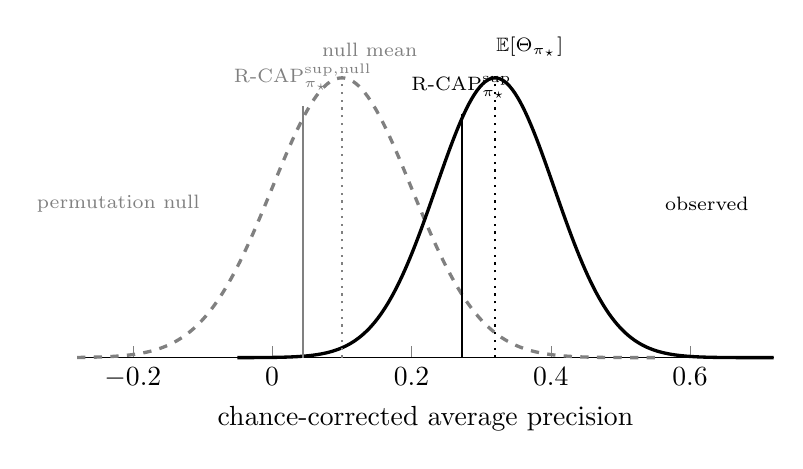
\begin{tikzpicture}
\begin{axis}[
  width=0.86\textwidth, height=6.2cm,
  xlabel={chance-corrected average precision},
  xmin=-0.28, xmax=0.72,
  ymin=0, ymax=1.30,
  axis y line=none,
  axis x line*=bottom,
  xtick={-0.2,0,0.2,0.4,0.6},
  clip=false,
  every axis plot/.append style={very thick},
]
% null replication distribution
\addplot[dashed, gray, domain=-0.28:0.55, samples=200]
  {exp(-((x-0.10)^2)/(2*0.100^2))};
% observed replication distribution
\addplot[solid, black, domain=-0.05:0.72, samples=200]
  {exp(-((x-0.32)^2)/(2*0.085^2))};
% markers
\draw[gray, dotted, thick] (axis cs:0.100,0) -- (axis cs:0.100,1.02);
\draw[gray, thick] (axis cs:0.044,0) -- (axis cs:0.044,0.90);
\draw[black, dotted, thick] (axis cs:0.320,0) -- (axis cs:0.320,1.02);
\draw[black, thick] (axis cs:0.272,0) -- (axis cs:0.272,0.87);
\node[gray, font=\scriptsize, anchor=south] at (axis cs:0.044,0.92) {$\RCAPnull$};
\node[gray, font=\scriptsize, anchor=south] at (axis cs:0.14,1.04) {null mean};
\node[font=\scriptsize, anchor=south] at (axis cs:0.272,0.89) {$\RCAP$};
\node[font=\scriptsize, anchor=south] at (axis cs:0.37,1.04) {$\E[\Theta_{\pi_\star}]$};
\node[gray, font=\scriptsize, anchor=east] at (axis cs:-0.09,0.55) {permutation null};
\node[font=\scriptsize, anchor=west] at (axis cs:0.55,0.55) {observed};
\end{axis}
\end{tikzpicture}
\caption{The replication distribution under the declared regime (solid) and under the permutation null (dashed). Each distribution is summarized by its mean and by the support functional, which sits below the mean by the disagreement penalty. The calibrated score in Equation~\eqref{eq:calibrated} measures the distance from $\RCAPnull$ to $\RCAP$ relative to the distance from $\RCAPnull$ to one. The null here lies above zero, which is the typical situation at small positive counts.}
\label{fig:distribution}
\end{figure}

A complete report should state:
\begin{itemize}
\item the reference prevalence $\pi_\star$;
\item the observed chance-corrected average precision $\Tpi(D_{\mathrm{obs}})$;
\item $\RCAPcalHat$ as the headline value, reported with $\RCAPHat$ and $\RCAPnullHat$;
\item the observed positive and negative counts;
\item the size and class-count design of each replicated evaluation;
\item the declared regime, including contexts held fixed and allowed to vary;
\item the method and unit used to generate replicates, and the unit of permutation;
\item the replicate count $B$, the permutation count $M$, and the Monte Carlo stability criterion;
\item any repeated model-development stages.
\end{itemize}

A report may read:
\begin{quote}
At a reference prevalence of $0.10$, R-CAP was $0.247$. The estimate cleared its measured chance level---the supported effect $\widehat{\operatorname{R\text{-}CAP}}{}^{\,\mathrm{sup}}_{0.10}$ was $0.270$ against a permutation null $\widehat{\operatorname{R\text{-}CAP}}{}^{\,\mathrm{sup,null}}_{0.10}$ of $0.031$, with a permutation $p$-value below $0.002$---so the calibrated value is read on its chance-to-perfect scale, zero being measured chance and one perfect separation. The observed chance-corrected average precision $\CAP_{0.10}(D_{\mathrm{obs}})$ was $0.340$. The evaluation contained 100 positive and 900 negative patients. The fixed-model regime held the target population, eligibility criteria, outcome definition, and measurement process fixed. Each of $5{,}000$ stratified bootstrap replicates sampled 100 positive and 900 negative patients with replacement from their respective observed classes. The null used $500$ permutations of the outcome labels across individual patients, each followed by the same $5{,}000$-replicate procedure. Both estimates were stable to three decimal places after doubling their respective Monte Carlo counts.
\end{quote}

Had the estimate not cleared its measured chance level---$\widehat{\operatorname{R\text{-}CAP}}{}^{\,\mathrm{sup}}_{0.10}$ at or below $\widehat{\operatorname{R\text{-}CAP}}{}^{\,\mathrm{sup,null}}_{0.10}$, equivalently a non-significant permutation $p$-value---the report would omit a calibrated headline, state the result as at or below measured chance, give the two supported quantities, and read the direction and magnitude of the effect from the signed observed effect $\CAP_{0.10}(D_{\mathrm{obs}})$ of Equation~\eqref{eq:T}, whose negative region is ordered and bounded, rather than from the calibrated scale.

When no single target prevalence is scientifically privileged, report
\[
\pi_\star
\longmapsto
\left\{
\Tpi(D_{\mathrm{obs}}),
\RCAPHat
\right\}
\]
over a prespecified plausible range, as in Figure~\ref{fig:profile}. This profile shows whether performance levels, disagreement penalties, or model orderings depend materially on the reference population.

\begin{figure}[ht]
\centering
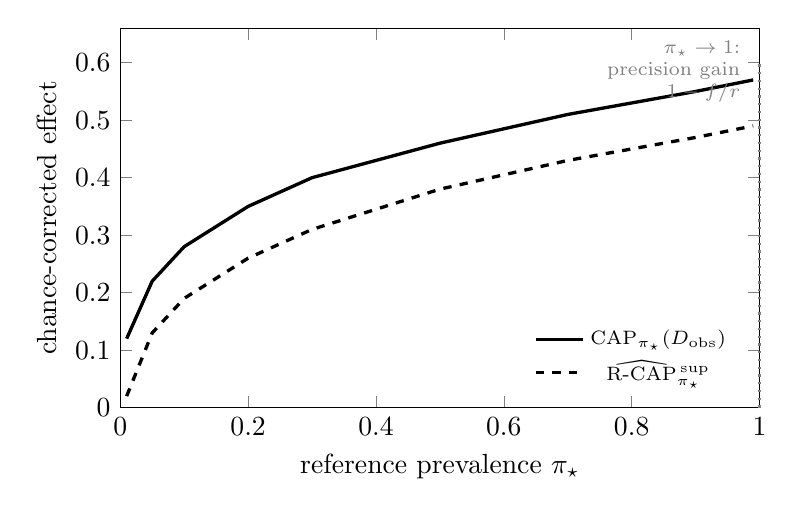
\begin{tikzpicture}
\begin{axis}[
  width=0.80\textwidth, height=6.4cm,
  xlabel={reference prevalence $\pi_\star$},
  ylabel={chance-corrected effect},
  xmin=0, xmax=1.0,
  ymin=0, ymax=0.66,
  xtick={0,0.2,0.4,0.6,0.8,1.0},
  ytick={0,0.1,0.2,0.3,0.4,0.5,0.6},
  legend pos=south east,
  legend style={font=\scriptsize, draw=none, fill=none},
  every axis plot/.append style={very thick},
  clip=false,
]
\addplot[black, mark=none] coordinates {
 (0.01,0.12) (0.05,0.22) (0.10,0.28) (0.20,0.35) (0.30,0.40)
 (0.50,0.46) (0.70,0.51) (0.90,0.55) (0.99,0.57)};
\addlegendentry{$\Tpi(D_{\mathrm{obs}})$}
\addplot[black, dashed, mark=none] coordinates {
 (0.01,0.02) (0.05,0.13) (0.10,0.19) (0.20,0.26) (0.30,0.31)
 (0.50,0.38) (0.70,0.43) (0.90,0.47) (0.99,0.49)};
\addlegendentry{$\RCAPHat$}
\draw[gray, dotted, thick] (axis cs:1.0,0) -- (axis cs:1.0,0.60);
\node[gray, font=\scriptsize, anchor=north east, align=right]
  at (axis cs:0.985,0.655) {$\pi_\star\to1$:\\ precision gain\\ $1-f/r$};
\end{axis}
\end{tikzpicture}
\caption{Illustrative reference-prevalence profile for one model. The observed effect and its supported counterpart are both nondecreasing in $\pi_\star$ for a better-than-chance ranker, by Equation~\eqref{eq:reference-prevalence-derivative}, and the disagreement penalty is largest where small changes in empirical false-positive rates matter most. The right-hand edge marks the limit at which the threshold-level integrand coincides with prevalence-free precision gain, per Section~\ref{sec:related-normalizations}. Values are illustrative.}
\label{fig:profile}
\end{figure}

\section{How evaluation size enters R-CAP\textsuperscript{sup}}

Return to two observed evaluations with chance-corrected average precision near $0.30$. Under the canonical estimator, the evaluation with 20 positive cases produces bootstrap repetitions containing 20 positives, while the evaluation with 20,000 positive cases produces repetitions containing 20,000 positives. Each also preserves its observed negative count. The values below illustrate replication distributions with the same mean repeated effect.

\begin{table}[ht]
\centering
\caption{Illustrative same-design repetitions with the same mean repeated effect.}
\label{tab:illustration}
\begin{tabular}{@{}lccc@{}}
\toprule
Evaluation & $\E[\Theta_{\pi_\star}]$ & $\tfrac12\E|\Theta_{\pi_\star,1}-\Theta_{\pi_\star,2}|$ & R-CAP\textsuperscript{sup} \\
\midrule
20 positive cases & $0.30$ & $0.12$ & $0.18$ \\
20,000 positive cases & $0.30$ & $0.01$ & $0.29$ \\
\bottomrule
\end{tabular}
\end{table}

The smaller evaluation loses more of its repeated effect because individual positive ranks have greater influence and its repetitions disagree more. The larger evaluation retains almost all of the same repeated effect. The numerical values are illustrative; the validation study must characterize their finite-sample behavior under specified score distributions.

Evaluation size also moves the chance level, and in the same direction. The smaller design has a larger disagreement penalty under permutation and a larger upward AP bias, so its null sits further from zero. Calibration removes the part of the difference in Table~\ref{tab:illustration} that is attributable to design rather than to the model.

R-CAP\textsuperscript{sup} contains no multiplicative sample-size factor. Positive and negative counts affect the score through the replication distribution induced by the repeated-evaluation design. As that distribution contracts around a value $t_0$,
\[
\RCAP\longrightarrow t_0.
\]
Additional information can reduce the disagreement penalty while leaving the limiting average-precision scale unchanged.

\section{Mathematical behavior and interpretive limits}
\label{sec:properties}

\subsection{Basic properties}

If $\Theta_{\pi_\star}=t$ with probability one, then $\RCAP=t$. No disagreement penalty remains when repetition is perfectly stable.

Since
\[
\min(\Theta_{\pi_\star,1},\Theta_{\pi_\star,2})
\leq
\frac{\Theta_{\pi_\star,1}+\Theta_{\pi_\star,2}}{2},
\]
we have
\[
\RCAP\leq\E[\Theta_{\pi_\star}].
\]
The supported score cannot exceed mean repeated performance.

If $L\leq\Theta_{\pi_\star}\leq U$, then
\[
L\leq\RCAP\leq U.
\]
For Equation~\eqref{eq:T}, take $L=-\pi_\star/(1-\pi_\star)$ and $U=1$.

If one replication distribution is everywhere better than another in the sense of first-order stochastic dominance, its R-CAP\textsuperscript{sup} cannot be smaller. Appendix~\ref{app:properties} gives proofs, a quantile representation, and the identification of $S_2$ within two established families.

The penalty depends on the full replication distribution. Two distributions can have the same mean and variance while assigning different probability to lower-tail failures. Their R-CAP\textsuperscript{sup} values can differ.

\subsection{Relation to a standard-error adjustment}

For a replication distribution that is approximately normal with standard deviation $\sigma$, $\E|\Theta_1-\Theta_2|=2\sigma/\sqrt{\pi}$, so
\begin{equation}
\RCAP
\approx
\E[\Theta_{\pi_\star}]-\frac{\sigma}{\sqrt{\pi}}
\approx
\E[\Theta_{\pi_\star}]-0.564\,\sigma .
\label{eq:se-approximation}
\end{equation}
To first order the estimate is the mean repeated effect shifted down by slightly more than half a replication standard error, which corresponds to roughly the $29$th percentile of the replication distribution. Equation~\eqref{eq:se-approximation} is a useful sanity check and should be stated rather than left for a reader to discover.

The minimum form is retained rather than replaced by an explicit standard-error adjustment for four reasons. It requires no distributional assumption. The constant $0.564$ is specific to normality and misstates the penalty for the skewed, discrete replication distributions produced by sparse positive counts and heavy ties, which is where the adjustment matters most. The same operator applies unchanged to paired differences in Section~\ref{sec:paired}, where a variance-based adjustment would require separate treatment of the correlation between models. And the population target in Equation~\eqref{eq:rcap} is defined through a first moment alone, so it exists under weaker conditions than a variance-based summary.

A reader who wants the effect estimate and its uncertainty separately should read them separately; the reporting requirements of Section~\ref{sec:reporting} supply both. The claim made for the supported score is not that it replaces an interval, but that it defines a single population functional with a stated replication meaning, which an interval does not.

\subsection{The support distribution and a survival level}

The support distribution has a simple form. Let $F$ be the distribution function of $\Theta_{\pi_\star}$ and $Q_{\pi_\star}$ its quantile function. Two independent repetitions give
\[
\Pr(M>m)=\{1-F(m)\}^2,
\qquad
M=\min\{\Theta_{\pi_\star,1},\Theta_{\pi_\star,2}\}.
\]
The level retained by both repetitions with frequency $\gamma$ is
\begin{equation}
m_\gamma=Q_{\pi_\star}(1-\sqrt{\gamma}).
\label{eq:survival-level}
\end{equation}
R-CAP\textsuperscript{sup} is the mean of $M$, and $m_\gamma$ is a low quantile of the same distribution. Under an approximately normal replication distribution the two track each other and R-CAP\textsuperscript{sup} sits near $m_{0.5}$. They separate when the distribution is lumpy. For a regime returning $\Theta_{\pi_\star}=1$ with probability $0.9$ and $0$ otherwise, R-CAP\textsuperscript{sup} is $0.81$ while $m_{0.9}$ is $0$. The gap $\RCAP-m_\gamma$ measures how much of the retained level depends on repetitions that can fail, and it is largest in the sparse-positive designs of Section~\ref{sec:sparse}.

The estimate is one index into the sorted replicate array of Appendix~\ref{app:computation},
\[
\widehat m_\gamma=t_{(\lceil B(1-\sqrt{\gamma})\rceil)}.
\]
It is a quantile of the estimated replication distribution and has the same status as $\RCAPHat$. It is not a confidence bound for a population parameter. A tail quantile is noisier than the mean and needs a larger $B$, and its estimate is least reliable in the sparse-positive regime where it is most informative. For general $K$ the same argument gives $m_\gamma^{(K)}=Q_{\pi_\star}(1-\gamma^{1/K})$, so $K$ and $\gamma$ traverse the same tail.

\subsection{Random ranking and the calibrated zero}

The chance-corrected effect $\Tpi$ places population random ranking at zero. The support functional does not inherit that property in finite samples, for the reasons given in Section~\ref{sec:calibration}: the upward bias of non-interpolated AP and the downward disagreement penalty partially cancel with a design-dependent residual of either sign. Chance is therefore located by permutation and removed by Equation~\eqref{eq:calibrated} rather than asserted.

The signed score preserves below-chance information. Clipping at zero changes finite-sample behavior near chance and should be avoided.

\subsection{Dependence on the reference prevalence}

$\RCAP$ is indexed by $\pi_\star$. Changing the reference prevalence changes the chance-corrected effect assigned to each repeated dataset and can change the center, shape, and lower tail of the replication distribution. A low reference prevalence can make early false positives and small changes in empirical false-positive rates especially influential. The resulting effect on disagreement depends on the score distributions, sample sizes, ties, and dependence structure. The permutation null must be recomputed at each $\pi_\star$ for which a calibrated value is reported.

Comparisons require a shared reference prevalence. Model rankings can reverse across values of $\pi_\star$, so a claim that one model has greater supported performance should state the reference prevalence or the range over which the ordering holds.

\subsection{Dependence on the declared regime}

$\RCAP$ is conditional on the size, class-count design, dependence structure, contextual variation, and model-development stages specified by $\Regime$. Changing any of these features changes the question being answered. Sensitivity analysis can compare plausible regimes, and external replications can test whether the stated invariances survive changes in site, time, assay, or case mix.

The name replication-adjusted describes the operator, not the breadth of the regime. Under the canonical estimator the repetitions are resamples of one held-out dataset, so the resulting value speaks to internal sampling variability and not to transportability across sites, periods, or assays. Only a regime that explicitly generates those sources of variation produces a score with external meaning.

\subsection{Sparse positive cases}
\label{sec:sparse}

Small positive counts make AP discrete and sensitive to individual ranks. They also limit empirical estimation of the positive score distribution, and they inflate both terms in Equation~\eqref{eq:two-distortions}. A low estimated R-CAP\textsuperscript{sup} can reflect weak repeated performance, broad variation across repetitions, limited information for estimating $\PRep$, or a combination of these features. Reporting $\RCAPnullHat$ alongside the estimate allows a reader to separate the design contribution from the model contribution. The permutation null shares this fragility. Its tail rests on the same small positive count, so the severity it measures is least reliable in the designs where the supported level is hardest to pin down.

\subsection{Replication count and severity}

The replication count $K$ sets how many independent repetitions a performance claim must survive. It is a severity parameter of the same kind as the declared regime and the reference prevalence, and it is declared with them. A stronger criterion uses
\[
S_K
=
\E\left[
\min(\Theta_{\pi_\star,1},\ldots,\Theta_{\pi_\star,K})
\right],
\]
which asks the claim to survive $K$ repetitions and places greater weight on the lower tail. Appendix~\ref{app:properties} gives the corresponding quantile weight. $S_K$ is decreasing in $K$ for any nondegenerate distribution. This is the content of the criterion. A claim asked to survive more repetitions is corroborated at a lower level.

The strict version asks a claim to survive every repetition the regime can produce. That level is $\lim_{K\to\infty}S_K$, the essential infimum of $\Theta_{\pi_\star}$. A finite sample cannot estimate it, since it estimates as the worst replicate and does not stabilize. Corroboration in practice is relative to a finite number of tests, and $K$ names that number. The default $K=2$ is the smallest count that expresses a repeated-performance criterion. Larger $K$ states a stricter claim and must be prespecified.

\subsection{Centering}

The definition in Equation~\eqref{eq:rcap} is replication-centered. A data-centered alternative preserves the observed point estimate and subtracts only the estimated penalty. Appendix~\ref{app:centering} states both forms and the grounds for preferring the first.

\section{Paired comparisons and a general support operator}
\label{sec:paired}

\subsection{Paired model comparison}

Suppose models $A$ and $B$ are evaluated on the same execution $D^{\mathrm{rep}}$ of the declared regime. Some repeated datasets may be easier for both models, while others may be harder. Their comparative performance within one evaluation is
\begin{equation}
\Delta_{\pi_\star}
=
\CAP_{A,\pi_\star}(D^{\mathrm{rep}})
-
\CAP_{B,\pi_\star}(D^{\mathrm{rep}}).
\label{eq:paired-difference}
\end{equation}
A positive value favors model $A$, a negative value favors model $B$, and zero represents equal chance-corrected average precision at reference prevalence $\pi_\star$.

Two independent executions of the regime produce
\[
\Delta_{\pi_\star,1},
\Delta_{\pi_\star,2}
\iid
P_{\mathrm{rep}}^{\Regime,\Delta_{\pi_\star}}.
\]
A superiority level $s$ is retained by both repetitions when
\[
s\leq \Delta_{\pi_\star,1},
\qquad
s\leq \Delta_{\pi_\star,2}.
\]
The largest such level is their minimum. Define supported superiority by
\begin{equation}
S_2(\Delta_{\pi_\star};\Regime)
=
\E_{\Regime}
\left[
\min\{
\Delta_{\pi_\star,1},
\Delta_{\pi_\star,2}
\}
\right].
\label{eq:paired}
\end{equation}
Using the minimum identity gives
\begin{equation}
S_2(\Delta_{\pi_\star};\Regime)
=
\E_{\Regime}[\Delta_{\pi_\star}]
-
\frac12
\E_{\Regime}
\left[
|\Delta_{\pi_\star,1}-\Delta_{\pi_\star,2}|
\right].
\label{eq:paired-decomposition}
\end{equation}
The first term is the expected advantage of model $A$ across repeated evaluations. The second term is half the expected disagreement between repeated advantages. A positive value retains a positive advantage for model $A$ under the two-repetition criterion. A nonpositive value supplies no positive supported-superiority claim for model $A$.

For estimation, evaluate both models on every replicated dataset $D^{(b)}$. Define
\[
t_{A,b}=\CAP_{A,\pi_\star}(D^{(b)}),
\qquad
t_{B,b}=\CAP_{B,\pi_\star}(D^{(b)}),
\qquad
\delta_b=t_{A,b}-t_{B,b}.
\]
The same resampled evaluation units and outcomes are used for both models within replicate $b$. This preserves the pairing and allows shared changes in evaluation difficulty to cancel in $\delta_b$. The all-pairs estimator is
\begin{equation}
\widehat S_{2,B}(\Delta_{\pi_\star};\Regime)
=
\frac{2}{B(B-1)}
\sum_{1\leq i<j\leq B}
\min(\delta_i,\delta_j).
\label{eq:paired-estimator}
\end{equation}

The paired difference supplies its own severity. It has an exact zero under equal performance, since $\Delta_{\pi_\star}=0$ identically when the two models produce the same ranking, and the finite-sample AP bias affects both models within the same replicate. The bias cancels in $\delta_b$ when the two models share threshold structure. When they do not, a permutation null exchanging model labels within replicates measures the residual, in the same way the outcome-label null measures chance for a single model. This severity comes from exchangeability of the model labels rather than from the outcome-label null of Section~\ref{sec:calibration}.

Subtracting the two marginal R-CAP\textsuperscript{sup} values can give a different result. Consider a regime with two equally likely evaluation contexts:
\begin{center}
\begin{tabular}{@{}lccc@{}}
\toprule
Context & $\CAP_{A,\pi_\star}$ & $\CAP_{B,\pi_\star}$ & $\Delta_{\pi_\star}$ \\
\midrule
1 & $0.90$ & $0.80$ & $0.10$ \\
2 & $0.40$ & $0.10$ & $0.30$ \\
\bottomrule
\end{tabular}
\end{center}
The paired difference takes values $0.10$ and $0.30$ with equal probability, which gives
\[
S_2(\Delta_{\pi_\star};\Regime)=0.15.
\]
The marginal support values are
\[
S_2(\CAP_{A,\pi_\star};\Regime)=0.525,
\qquad
S_2(\CAP_{B,\pi_\star};\Regime)=0.275,
\]
so their difference is $0.25$. Subtracting marginal support values compares two separate replication summaries. Equation~\eqref{eq:paired} evaluates the advantage of model $A$ within each repeated dataset and then applies the support criterion to that advantage. It follows that marginal R-CAP\textsuperscript{sup} values reported in separate studies cannot be differenced to infer supported superiority; a paired comparison requires joint evaluation on common replicates.

\subsection{The general support operator}

Let $T(D)$ be any scalar performance effect defined on a common scale, with larger values representing better performance. Under a declared evaluation-generating regime $\Regime$, let
\[
T_1,T_2
\iid
P_{\mathrm{rep}}^{\Regime,T}
\]
be the effects from two independent executions. Define
\begin{equation}
S_2(T;\Regime)
=
\E_{\Regime}
\left[
\min(T_1,T_2)
\right].
\label{eq:general}
\end{equation}
The operator maps a replication distribution to the average performance level retained by two repetitions. It also has the disagreement form
\begin{equation}
S_2(T;\Regime)
=
\E_{\Regime}[T]
-
\frac12
\E_{\Regime}[|T_1-T_2|].
\label{eq:general-decomposition}
\end{equation}

The operator is not new. Equation~\eqref{eq:general-decomposition} is the difference of the first two L-moments, $\lambda_1-\lambda_2$, and Equation~\eqref{eq:quantile} below identifies $S_K$ as a member of the dual-power family of distortion risk measures. Appendix~\ref{app:families} records the properties that follow immediately from that identification, several of which are proved directly elsewhere in this document. The mathematics supplies the properties. The application supplies the meaning. $S_K$ is used here as a corroboration criterion on a prevalence-standardized, chance-corrected precision-recall effect, evaluated under a declared regime and calibrated against a permutation null. The two severity axes give the number its scientific content.

R-CAP\textsuperscript{sup} is that application:
\begin{equation}
\RCAPfull
=
S_2(\CAP_{\pi_\star};\Regime).
\label{eq:rcap-as-support-operator}
\end{equation}
The transformation $\CAP_{\pi_\star}$ supplies the prevalence-indexed performance scale. The operator $S_2$ supplies the replication-support criterion. The permutation null of Section~\ref{sec:calibration} supplies the origin.

Other choices of $T$ can produce supported AUROC, correlation, $R^2$, subgroup contrasts, or paired improvements. The direction of the scale must be defined so that larger values represent better performance. For a loss $L(D)$, one may use $T(D)=-L(D)$. For comparison of two models by loss, one may use
\[
T(D)=L_B(D)-L_A(D),
\]
so that positive values favor model $A$. The evaluation-generating regime and the estimation procedure must represent the sources of variation relevant to the resulting claim, and any effect scale with a finite-sample bias at its own null requires the same calibration step.

\section{Conclusion}

Average precision describes positive retrieval and selected-set purity. Its value depends on positive-class prevalence, and one finite evaluation can provide limited support for the observed result. Precision odds factor into prior odds and a likelihood ratio, so prevalence enters through exactly one term. Declaring a reference prevalence $\pi_\star$ replaces that term with a scientifically chosen value, in contrast to prevalence-free normalizations that divide it out. Chance correction then produces the chance-corrected average precision
\[
\Tpi(D)
=
\frac{\AP_{\pi_\star}(D)-\pi_\star}{1-\pi_\star}.
\]
The choice of $\pi_\star$ remains part of the scientific claim. When several target populations are relevant, a reference-prevalence profile can accompany the primary value.

The replication-support operator acts on any scalar performance effect $T(D)$ for which larger values represent better performance:
\[
S_2(T;\Regime)
=
\E_{\Regime}
\left[
\min(T_1,T_2)
\right].
\]
The evaluation-generating regime $\Regime$ specifies what constitutes a complete repetition. It includes the sample size, class-count design, dependence structure, target context, measurement process, and model-development stages that recur. The operator therefore describes the performance level that survives two independent executions of a declared evaluation design. Survival under replication is one axis of severity. The permutation null of the calibration step is the second, a measured chance level under the same regime.

R-CAP\textsuperscript{sup} applies this operator to the prevalence-indexed chance-corrected average precision:
\begin{equation}
\RCAPfull
=
S_2(\CAP_{\pi_\star};\Regime).
\label{eq:conclusion-rcap-operator}
\end{equation}
It equals expected repeated performance at $\pi_\star$ minus half the expected disagreement between repetitions. R-CAP\textsuperscript{sup} is a property of the performance functional, reference population, and evaluation-generating regime together. It is not a property of the fitted model alone. Applying the same operator to within-replication performance differences gives a paired measure of supported model superiority that cannot be recovered by differencing marginal values.

The population quantity in Equation~\eqref{eq:conclusion-rcap-operator} is generally unknown. For a fixed model evaluated on independent or held-out data, the canonical estimate uses a stratified $n$-out-of-$n$ bootstrap. Each replicate preserves the observed positive and negative counts and represents another evaluation of the same design under the empirical class-conditional distributions. Broader regimes require replication procedures that represent their additional sources of variation.

Analytic chance correction is not sufficient at finite sample sizes. Non-interpolated average precision is upward biased under random ranking, the minimum imposes a downward disagreement penalty, and the residual after cancellation depends on the design. The chance level is therefore measured by a permutation null executed under the same declared regime, and the calibrated score
\[
\RCAPcalHat
=
\frac{\RCAPHat-\RCAPnullHat}{1-\RCAPnullHat}
\]
restores zero to chance while retaining an exact ceiling at perfect separation. The calibrated effect is the primary reported value, and the observed effect and the supported effect are reported together with it.

Simulation and empirical study remain necessary to establish finite-sample behavior, sensitivity to sparse positives, robustness to dependence and regime misspecification, the adequacy of the canonical bootstrap, and the stability of the permutation null under broad regimes. The proposal supplies a defined population target, an operational estimator for a common setting, and a measured origin for the resulting scale. Reporting the observed effect with its replication-supported and calibrated counterparts separates the performance seen in one dataset from the performance claim sustained by repetition of the declared evaluation design.

\newpage

\begin{thebibliography}{9}

\bibitem{bouckaert2004estimating}
Bouckaert, R. R. (2004).
Estimating replicability of classifier learning experiments.
In \emph{Proceedings of the 21st International Conference on Machine Learning}, pages 137--144.

\bibitem{elkan2001foundations}
Elkan, C. (2001).
The foundations of cost-sensitive learning.
In \emph{Proceedings of the 17th International Joint Conference on Artificial Intelligence}, pages 973--978.

\bibitem{flach2015prg}
Flach, P. A. and Kull, M. (2015).
Precision-Recall-Gain curves: PR analysis done right.
In Cortes, C., Lawrence, N. D., Lee, D. D., Sugiyama, M., and Garnett, R., editors,
\emph{Advances in Neural Information Processing Systems 28}, pages 838--846.

\bibitem{hoeffding1948ustat}
Hoeffding, W. (1948).
A class of statistics with asymptotically normal distribution.
\emph{Annals of Mathematical Statistics}, 19(3):293--325.

\bibitem{hosking1990lmoments}
Hosking, J. R. M. (1990).
L-moments: analysis and estimation of distributions using linear combinations of order statistics.
\emph{Journal of the Royal Statistical Society, Series B}, 52(1):105--124.

\bibitem{mayo1996error}
Mayo, D. G. (1996).
\emph{Error and the Growth of Experimental Knowledge}.
University of Chicago Press.

\bibitem{nadeau2003inference}
Nadeau, C. and Bengio, Y. (2003).
Inference for the generalization error.
\emph{Machine Learning}, 52(3):239--281.

\bibitem{ojala2010permutation}
Ojala, M. and Garriga, G. C. (2010).
Permutation tests for studying classifier performance.
\emph{Journal of Machine Learning Research}, 11:1833--1863.

\bibitem{popper1959logic}
Popper, K. R. (1959).
\emph{The Logic of Scientific Discovery}.
Hutchinson, London.

\bibitem{wang1996premium}
Wang, S. S. (1996).
Premium calculation by transforming the layer premium density.
\emph{ASTIN Bulletin}, 26(1):71--92.

\end{thebibliography}

\addtocontents{toc}{\protect\setcounter{tocdepth}{0}}

\newpage
\appendix

\section{Reference-prevalence average precision}
\label{app:prevalence}

\subsection{Population transformation}

Let $Y\in\{0,1\}$ be the outcome and let $S$ be a ranking score. At threshold $c$, define
\[
r(c)=\Pr(S\geq c\mid Y=1),
\qquad
f(c)=\Pr(S\geq c\mid Y=0).
\]
These quantities are the true-positive and false-positive rates. For prevalence $\pi$, precision is
\[
p_{\pi}(c)
=
\frac{\pi r(c)}{\pi r(c)+(1-\pi)f(c)}.
\]

Suppose an evaluation has prevalence $\pi$ and threshold-specific precision $p(c)$. The precision implied by reference prevalence $\pi_\star$ is
\begin{equation}
p_{\pi_\star}(c)
=
\frac{(\pi_\star/\pi)p(c)}
{(\pi_\star/\pi)p(c)
+
\{(1-\pi_\star)/(1-\pi)\}\{1-p(c)\}}.
\label{eq:precision-transform}
\end{equation}

The transformation keeps $r(c)$ and $f(c)$ fixed. It changes the class prior used to calculate precision. In odds form it is a single multiplication,
\[
\frac{p_{\pi_\star}}{1-p_{\pi_\star}}
=
\frac{\pi_\star(1-\pi)}{\pi(1-\pi_\star)}
\cdot
\frac{p}{1-p},
\]
which is Equation~\eqref{eq:odds} with the prior odds exchanged.

\subsection{Precision gain and the prevalence-free limit}
\label{app:precg}

Let $\operatorname{precG}=(p-\pi)/\{(1-\pi)p\}$ with $p=\pi r/\{\pi r+(1-\pi)f\}$ and write $D=\pi r+(1-\pi)f$. Then
\[
p-\pi
=
\frac{\pi r-\pi D}{D}
=
\frac{\pi\{r-\pi r-(1-\pi)f\}}{D}
=
\frac{\pi(1-\pi)(r-f)}{D},
\qquad
(1-\pi)p
=
\frac{(1-\pi)\pi r}{D},
\]
so
\[
\operatorname{precG}
=
\frac{\pi(1-\pi)(r-f)/D}{(1-\pi)\pi r/D}
=
\frac{r-f}{r}
=
1-\frac{f}{r}.
\]
The prevalence terms cancel identically. Comparing with Equation~\eqref{eq:precg-limit} confirms that precision gain is the $\pi_\star\to1$ limit of the threshold-level integrand used here.

The corresponding recall gain is $\operatorname{recG}=(r-\pi)/\{(1-\pi)r\}$, which vanishes at $r=\pi$ and equals one at $r=1$, with
\[
\frac{d\operatorname{recG}}{dr}
=
\frac{\pi}{(1-\pi)r^{2}} .
\]
Integrating precision gain against $d\operatorname{recG}$ therefore weights the region $r\in[\pi,1]$ proportionally to $r^{-2}$. Integrating the chance-corrected precision of Equation~\eqref{eq:threshold-normalized-effect} against $dr$ does not. The two summaries coincide at the threshold level in the limit and differ as integrals for every $\pi_\star$.

\subsection{Empirical definition}

Let
\[
D=\{(s_i,y_i)\}_{i=1}^{n},
\qquad y_i\in\{0,1\},
\]
with $n_+=\sum_i y_i>0$ and $n_-=n-n_+>0$. Let
\[
c_1>c_2>\cdots>c_K
\]
be the distinct observed score values. Threshold $k$ selects every observation with $s_i\geq c_k$. Define
\[
\operatorname{TP}_k
=
\sum_{i=1}^{n}\mathbf{1}\{y_i=1,\ s_i\geq c_k\},
\qquad
\operatorname{FP}_k
=
\sum_{i=1}^{n}\mathbf{1}\{y_i=0,\ s_i\geq c_k\},
\]
and
\[
r_k=\frac{\operatorname{TP}_k}{n_+},
\qquad
f_k=\frac{\operatorname{FP}_k}{n_-}.
\]
Reference-prevalence precision at the threshold is
\begin{equation}
p_{\pi_\star,k}
=
\frac{\pi_\star r_k}
{\pi_\star r_k+(1-\pi_\star)f_k}.
\label{eq:empirical-reference-precision}
\end{equation}
Set $r_0=0$. Reference-prevalence average precision is
\begin{equation}
\AP_{\pi_\star}(D)
=
\sum_{k=1}^{K}
(r_k-r_{k-1})p_{\pi_\star,k}.
\label{eq:standardized-ap}
\end{equation}
A threshold that adds only negative cases has $r_k-r_{k-1}=0$. Its false positives still affect precision at later thresholds.

Equation~\eqref{eq:standardized-ap} evaluates precision at thresholds determined by the observed positions of positive cases. This is the source of the upward bias $\beta$ in Equation~\eqref{eq:two-distortions}, since those positions are favourably placed by chance more often than the population baseline implies.

\subsection{Equal scores}

Equal scores form one threshold block. Every observation in the block enters the selected set at the same threshold. This rule uses only distinctions made by the model.

Consider the scores and classes
\[
(0.90,+),\quad(0.70,+),\quad(0.70,-),\quad(0.20,-).
\]
An arbitrary ordering of the two middle cases can produce ordinary AP of $1$ or $5/6$. The model assigns them the same score. Under the block rule, both enter at threshold $0.70$. Precision is then $2/3$ and recall rises from $1/2$ to $1$. Equation~\eqref{eq:standardized-ap}, with the observed prevalence used as the reference prevalence, gives
\[
\AP
=
\frac12(1)+\frac12\left(\frac23\right)
=
\frac56.
\]
Use the model's unrounded numerical scores when they are available. Rounding before evaluation can create ties that were absent from the model output. Because the permutation null of Section~\ref{sec:calibration} preserves the score multiset, it also preserves the tie structure, and the resulting chance level reflects the ties actually present.

\subsection{Average-precision convention}

Equation~\eqref{eq:standardized-ap} uses non-interpolated stepwise average precision. Each increase in recall receives the precision at the threshold that produced it.

Trapezoidal PR area joins adjacent operating points with straight lines. Interpolated AP replaces the empirical precision sequence with a precision envelope. These conventions can give different finite-sample values, and they carry different chance levels. All R-CAP calculations in this document use the stepwise convention in Equation~\eqref{eq:standardized-ap}.

\subsection{Equivalent weighted implementation}

The same quantity can be calculated by assigning each observation the class weight
\begin{equation}
w_i
=
\begin{cases}
\pi_\star/n_+, & y_i=1,\\[4pt]
(1-\pi_\star)/n_-, & y_i=0.
\end{cases}
\label{eq:reference-weights}
\end{equation}
The positive weights sum to $\pi_\star$. The negative weights sum to $1-\pi_\star$. At threshold $k$, weighted precision is
\[
\frac{(\pi_\star/n_+)\operatorname{TP}_k}
{(\pi_\star/n_+)\operatorname{TP}_k
+
\{(1-\pi_\star)/n_-\}\operatorname{FP}_k}
=
p_{\pi_\star,k},
\]
and weighted recall is
\[
\frac{(\pi_\star/n_+)\operatorname{TP}_k}{\pi_\star}
=
r_k.
\]
A weighted AP routine therefore returns $\AP_{\pi_\star}(D)$ when it groups equal scores and uses non-interpolated stepwise AP.

Under the canonical stratified bootstrap, $n_+^{(b)}=n_+$ and $n_-^{(b)}=n_-$ for every replicate. Recalculate the threshold counts, $r_k^{(b)}$, and $f_k^{(b)}$ within each replicate while keeping $\pi_\star$ fixed. When the declared regime allows class counts to vary, use the replicate-specific $n_+^{(b)}$ and $n_-^{(b)}$ in the class weights. Each replicate must contain both outcome classes. A procedure that drops zero-class executions changes the regime-relative replication distribution and requires an explicit conditional estimand.

The prevalence transformation assumes that the class-conditional score distributions remain relevant at $\pi_\star$. Prior-probability shift satisfies this condition. Changes in case mix within either class can violate it.

\section{Properties of the support functional}
\label{app:properties}

\subsection{Common support}

\begin{proposition}
For realized values $t_1$ and $t_2$, the largest real number that does not exceed either value is $\min(t_1,t_2)$.
\end{proposition}

\begin{proof}
Every admissible level $s$ satisfies $s\leq t_1$ and $s\leq t_2$, so $s\leq\min(t_1,t_2)$. The value $\min(t_1,t_2)$ satisfies both inequalities. It is therefore the largest admissible level.
\end{proof}

\subsection{Disagreement decomposition}

\begin{proposition}
If $\Theta_{\pi_\star,1}$ and $\Theta_{\pi_\star,2}$ are independent and identically distributed with finite first moment, then
\[
\E\min(\Theta_{\pi_\star,1},\Theta_{\pi_\star,2})
=
\E\Theta_{\pi_\star}
-
\frac12
\E|\Theta_{\pi_\star,1}-\Theta_{\pi_\star,2}|.
\]
\end{proposition}

\begin{proof}
Use
\[
\min(a,b)=\frac{a+b-|a-b|}{2}
\]
and take expectations. Identical distributions give
\[
\E\Theta_{\pi_\star,1}
=
\E\Theta_{\pi_\star,2}
=
\E\Theta_{\pi_\star}.
\]
\end{proof}

\subsection{Quantile representation}

Let $Q_{\pi_\star}(u)$ be a generalized quantile function of $\Theta_{\pi_\star}$. If $\E|\Theta_{\pi_\star}|<\infty$, then
\begin{equation}
S_K
=
\int_0^1 K(1-u)^{K-1}Q_{\pi_\star}(u)\,du,
\qquad
\RCAP
=
\int_0^1 2(1-u)Q_{\pi_\star}(u)\,du.
\label{eq:quantile}
\end{equation}

To see this, write $\Theta_{\pi_\star,i}=Q_{\pi_\star}(U_i)$ for independent $U_i\sim\operatorname{Uniform}(0,1)$. Since $Q_{\pi_\star}$ is nondecreasing,
\[
\min_i\{Q_{\pi_\star}(U_i)\}
=
Q_{\pi_\star}\{\min_i(U_i)\}.
\]
The minimum of $K$ independent uniform variables has density $K(1-u)^{K-1}$ on $(0,1)$.

Ordinary expectation weights quantiles uniformly. Equation~\eqref{eq:quantile} gives greater weight to lower quantiles through the $K$-repetition criterion, and the weighting becomes more concentrated on the lower tail as $K$ increases.

\subsection{Two established families}
\label{app:families}

The operator coincides with objects defined elsewhere, and the identification supplies several properties without separate proof.

\paragraph{L-moments.}
The first two L-moments of a distribution~\cite{hosking1990lmoments} are $\lambda_1=\E[T]$ and $\lambda_2=\tfrac12\E|T_1-T_2|$, the latter being half the Gini mean difference. Equation~\eqref{eq:general-decomposition} is therefore the exact identity
\[
S_2(T;\Regime)=\lambda_1-\lambda_2 .
\]
L-moment estimators are linear in order statistics, which is the origin of the sorted-sum form in Appendix~\ref{app:computation}, and they exist whenever the first moment does.

\paragraph{Distortion risk measures.}
Equation~\eqref{eq:quantile} expresses $S_K$ as a distortion measure with distortion function $g(u)=1-(1-u)^{K}$, a member of the dual-power family in the sense of Wang~\cite{wang1996premium}. Because $g$ is concave, the following hold immediately: monotonicity with respect to first-order stochastic dominance; translation equivariance, $S_2(T+c)=S_2(T)+c$; positive homogeneity, $S_2(aT)=aS_2(T)$ for $a>0$; comonotone additivity; and concavity as a functional of the gain variable. The monotonicity result proved directly below is the first of these.

\paragraph{U-statistics.}
Equation~\eqref{eq:uestimator} is a U-statistic of degree two with kernel $h(t_i,t_j)=\min(t_i,t_j)$, so its behavior as $B$ grows follows from the theory of Hoeffding~\cite{hoeffding1948ustat}, with variance governed by the projection $h_1(t)=\E[\min(t,T)]$. This concerns Monte Carlo accuracy for fixed $\PRepHat$ and not the statistical information in $D_{\mathrm{obs}}$.

\subsection{Conservatism and consistency}

The inequality
\[
\min(\Theta_{\pi_\star,1},\Theta_{\pi_\star,2})
\leq
\frac{\Theta_{\pi_\star,1}+\Theta_{\pi_\star,2}}{2}
\]
gives $\RCAP\leq\E\Theta_{\pi_\star}$.

Suppose $\Theta_{\pi_\star,n}\to t_0$ in probability and all $\Theta_{\pi_\star,n}$ lie in a common bounded interval. Then two independent copies satisfy
\[
\min(\Theta_{\pi_\star,n,1},\Theta_{\pi_\star,n,2})\to t_0
\]
in probability. Bounded convergence gives
\[
\E\min(\Theta_{\pi_\star,n,1},\Theta_{\pi_\star,n,2})\to t_0.
\]
Under the same conditions the permutation null converges to the population chance level, so the calibrated score in Equation~\eqref{eq:calibrated} converges to $t_0$ whenever the population chance level is zero.

\subsection{Monotonicity}

Let $Q_A$ and $Q_B$ be quantile functions with $Q_A(u)\geq Q_B(u)$ for all $u\in(0,1)$. Equation~\eqref{eq:quantile} gives
\[
S_2(A)\geq S_2(B).
\]
This condition is first-order stochastic dominance.

\subsection{Centering}
\label{app:centering}

The primary definition is replication-centered:
\[
S_{\mathrm{rep}}
=
\E_{\mathrm{rep}}
\left[
\min(\Theta_{\pi_\star,1},\Theta_{\pi_\star,2})
\right].
\]
It includes the location of expected repeated performance and the disagreement between repetitions.

A data-centered alternative is
\[
S_{\mathrm{obs}}
=
\Tpi(D_{\mathrm{obs}})
-
\frac12
\E_{\PRepHat}
\left[
|\Theta_{\pi_\star,1}-\Theta_{\pi_\star,2}|
\mid D_{\mathrm{obs}}
\right].
\]
It preserves the observed point estimate and subtracts the estimated disagreement penalty. The replication-centered form is preferred because it matches the target of expected repeated performance and because it is a functional of a single declared distribution, whereas the data-centered form mixes a realized value with a resampling summary. Simulation should compare both forms under finite samples and model misspecification.

\section{Efficient computation}
\label{app:computation}

Let $t_1,\ldots,t_B$ be independent draws from the distribution whose support functional is being calculated, usually $\PRepHat(\cdot\mid D_{\mathrm{obs}})$. Sort them so that
\[
t_{(1)}\leq t_{(2)}\leq\cdots\leq t_{(B)}.
\]
The value $t_{(i)}$ is the minimum in each pair formed with one of the $B-i$ larger values. Equation~\eqref{eq:uestimator} becomes
\begin{equation}
\RCAPHatB
=
\frac{2}{B(B-1)}
\sum_{i=1}^{B-1}(B-i)t_{(i)}.
\label{eq:sorted}
\end{equation}

This calculation requires sorting followed by one weighted sum. Its computational cost is $O(B\log B)$.

A direct implementation can use the following sequence:

\begin{enumerate}
\item Store the $B$ replicated chance-corrected average-precision values.
\item Sort them in ascending order.
\item Multiply $t_{(i)}$ by $B-i$ for $i=1,\ldots,B-1$.
\item Sum the products and multiply by $2/[B(B-1)]$.
\end{enumerate}

For general $K$, the same argument gives
\[
\widehat S_{K,B}
=
\binom{B}{K}^{-1}
\sum_{i=1}^{B-K+1}
\binom{B-i}{K-1}
t_{(i)},
\]
since $t_{(i)}$ is the minimum of exactly $\binom{B-i}{K-1}$ subsets of size $K$.

The calibrated score of Section~\ref{sec:calibration} repeats this calculation once per permutation, giving total cost $O(MB\log B)$ together with $M$ evaluations of the resampling step. The permutations are mutually independent and parallelize without communication, and $M$ between $200$ and $500$ suffices for the location estimate $\RCAPnullHat$. A small permutation $p$-value requires larger $M$, and regimes that repeat model development multiply the cost by the training time rather than by the sorting cost.

\end{document}